\chapter{CoCo Structure}

This chapter explains the nature of CoCos, a new member in the family of hybrid securities. In the following, the general structure of these new instruments will be explained (section \ref{definitioncocos}) including characteristic design features among others their trigger (section \ref{triggermechanism}) and loss-absorption mechanism (section \ref{lossabsorption}).

\section{Definition}\label{definitioncocos}

The term CoCo is used to describe a new hybrid capital instrument with an automatic conversion mechanism which morphs debt into equity when the financial soundness of the issuer is at stake. A write-down of the notional is also a viable loss-absorption mechanism to recapitalize the distressed bank. Generally, the loss-absorption mechanism is activated if a predefined trigger level is breached. \citep{de2011pricing, zahres2011contingent}. In this context, figure \ref{figure:anatomy} provides an overview of major design characteristics. Exactly  these anatomic aspects will be explained in the subsequent sections.\\

\begin{figure}[ht]
	\centering
	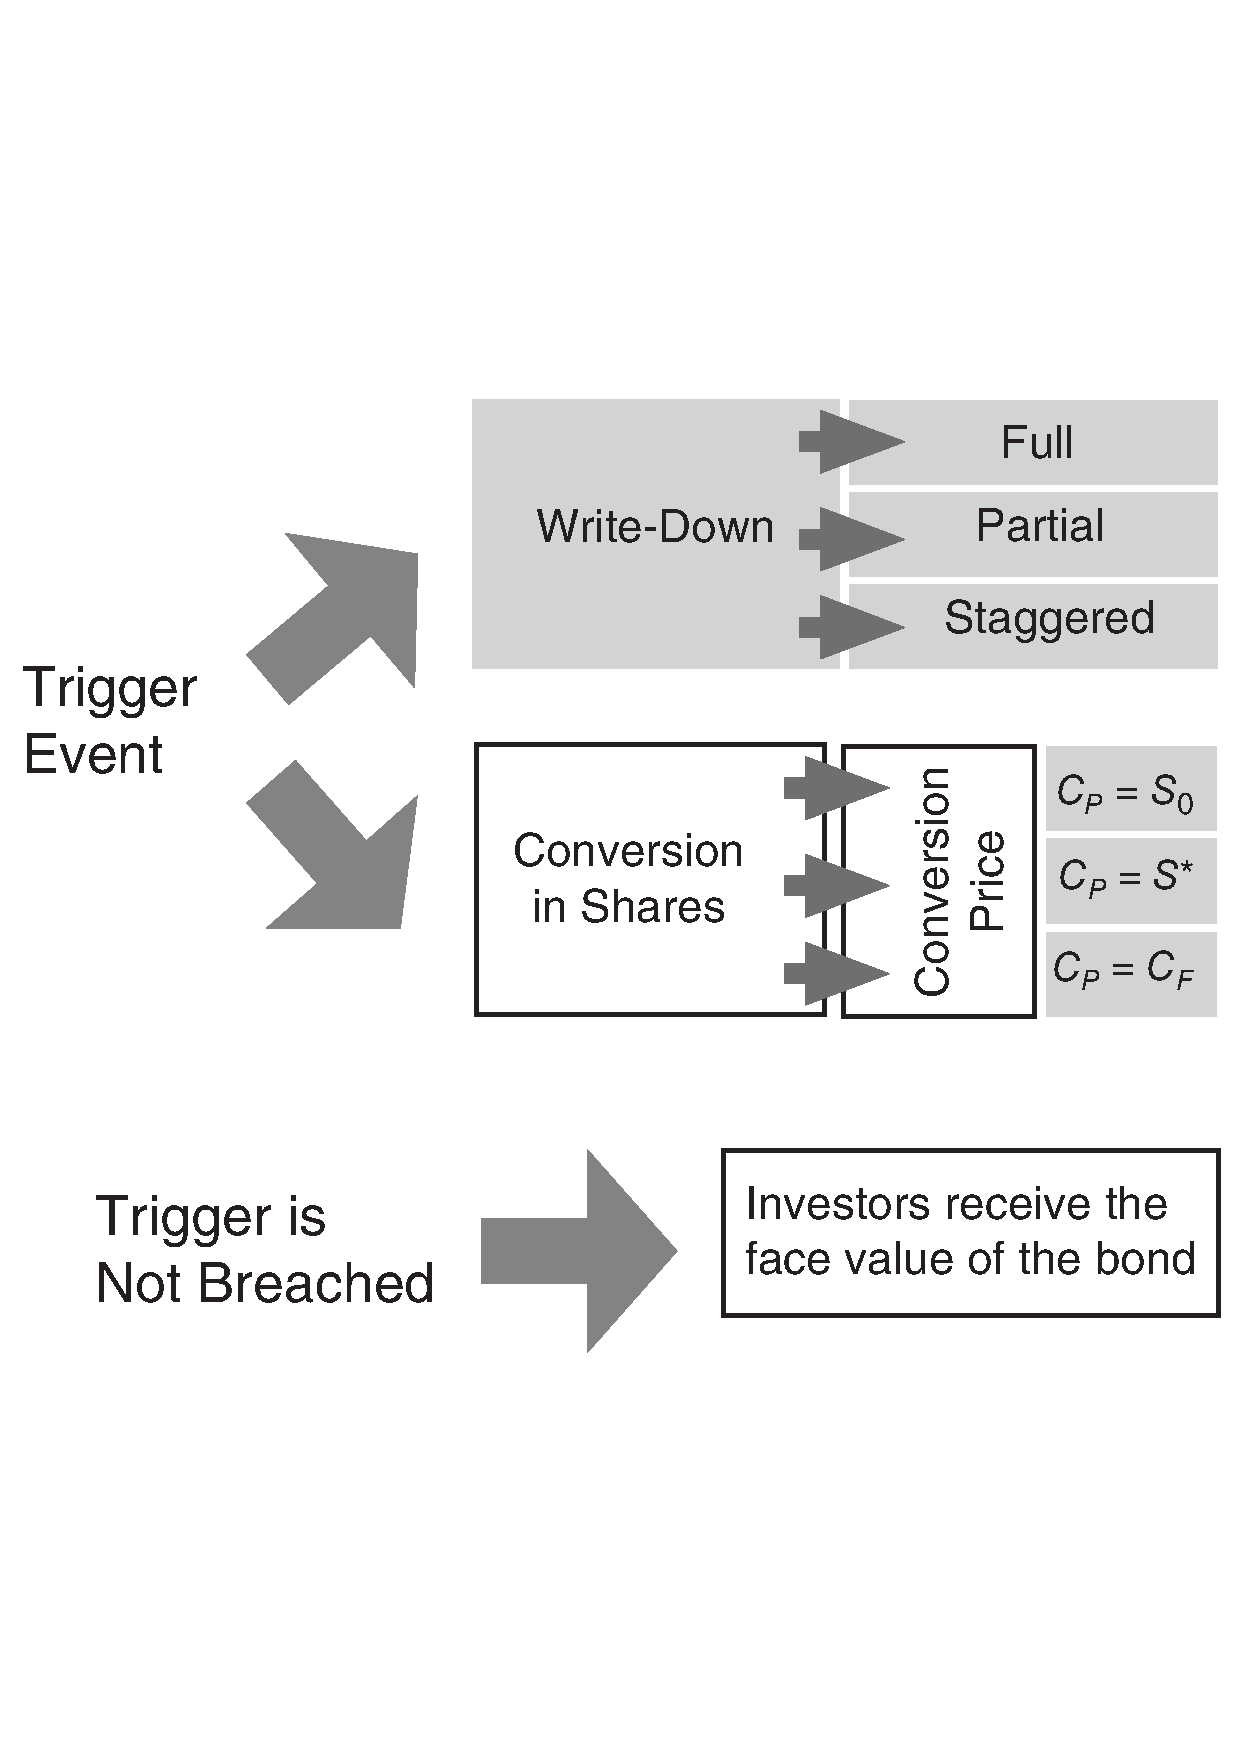
\includegraphics[trim=0.6cm 7.05cm 0.9cm 7cm, scale = 0.32]{media/anatomy} \par
	\caption[Anatomy of CoCos]{Anatomy of CoCos \citep{de2014handbook}}
	\label{figure:anatomy}
\end{figure}
CoCos are particularly interesting from the perspective of a regulatory authority because they might mitigate externalization costs of insolvencies and frictions due to spill-over effects. In times of distress, stakeholders might question the financial viability of the respective financial institute. Yet, the major advantage of CoCos is that a distressed bank does not have to approach new investors to issue new capital in extremely though times as everything happens automatically. \citep{de2011pricing}\\ 

In 2009, the Lloyds Banking Group was the first financial institute which issued this new financial instrument. In an exchange offer, they asked hybrid debt holders to swap their holdings into CoCos. \citep{de2011pricing} In 2010, the Basel Committee on Banking Supervision (BCBS) provided further impetus to the use of this instrument when it disclosed its proposal to ensure the loss absorbency of regulatory capital at the point of non-viability. CoCos fit into their line of  argumentation that regulatory capital instruments have to be capable of absorbing financial losses in gone-concern phases. \citep{basel2010proposal}

%\begin{figure}[ht]
%	\centering
%	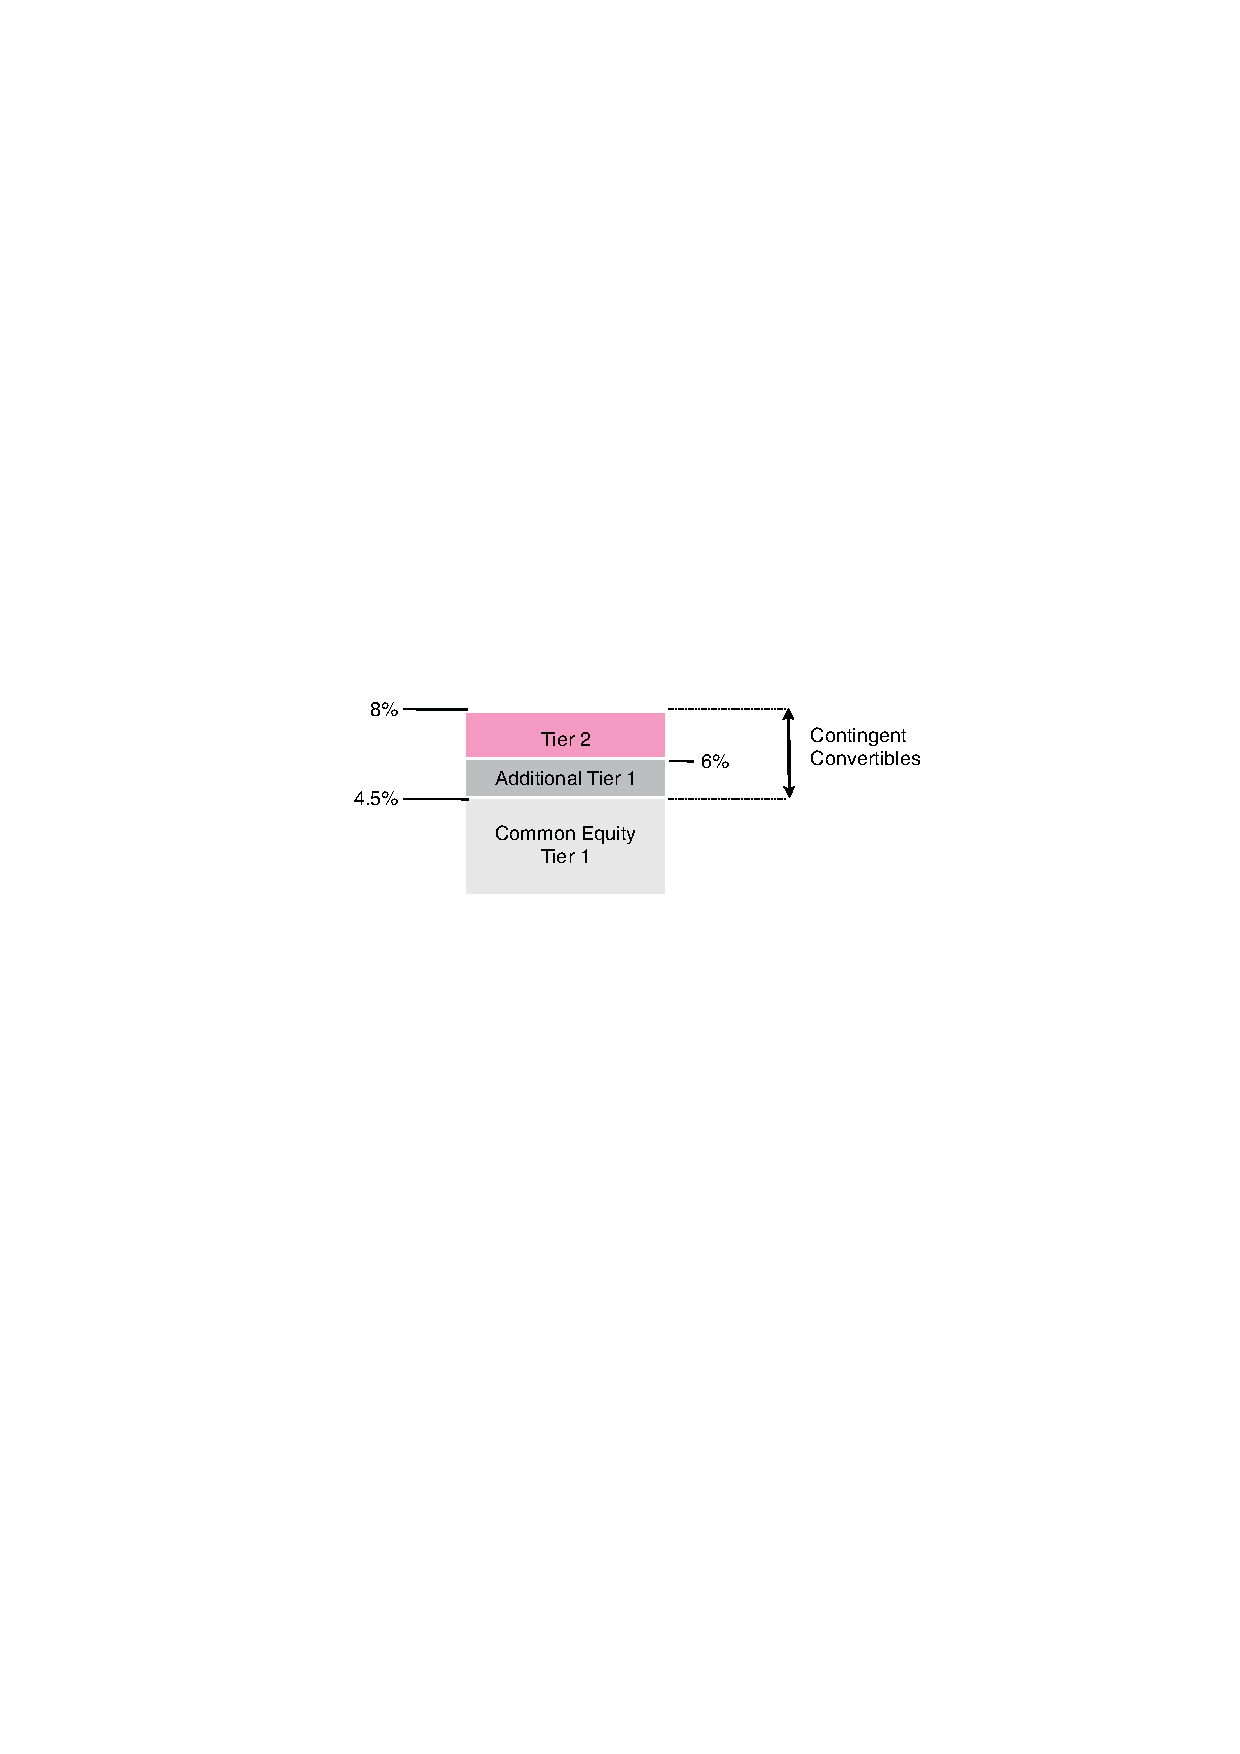
\includegraphics[trim=0.1cm 0.1cm 0.2cm 0.1cm, scale = 1]{media/basel3} \par
%	\caption[CoCos under Basel III]{CoCos under Basel III \citep{de2014handbook}}
%\end{figure}

%The term CoCo is used to describe a new type of convertible bond that is automatically converted into a predetermined amount of shares when a predefined trigger is breached. Since this type of bond is transformed into equity upon conversion, it would be available for further loss-absorption and therefore satisfies the new regulatory requirements of hybrid capital instruments. \citep{zahres2011contingent}

\section{Trigger} \label{triggermechanism}

The trigger is a key design element of a CoCo which initializes the loss-absorption mechanism. In the following sections, four different trigger mechanisms will be described: accounting triggers, market triggers, regulatory triggers and multi-variate triggers. %Generally one can evaluate the trigger design based on the criteria as summarized by \citet{erismann2015pricing}. %The concept of an accounting trigger will be illustrated in section \ref{accountingtrigger} followed by the market trigger in section \ref{markettrigger}. Additionally, the regulatory trigger will be detailed in section \ref{regulatorytrigger} and the multi-variate trigger will be explained in section \ref{multivariatetrigger}.

%\begin{itemize}
%\renewcommand\labelitemi{--}
%\item \textbf{Clarity}:  The trigger mechanism should be universally applicable irrespective of the jurisdiction in which the CoCo is traded.
%\item \textbf{Fixedness}: The definition of a CoCo's trigger should remain the same until maturity.
%\item \textbf{Frequency}: Data to which the trigger is linked should be updated at frequent intervals.
%\item \textbf{Objectiveness}: The trigger mechanism should be based on observable and well-known facts. Their should be no room for subjectivity.
%\item \textbf{Publicity}: Data concerning the trigger should be open to the general view of all market participants at the same time. This needs to be possible without concealment, thereby reducing the chance of manipulation.
%\end{itemize}

%\begin{table}[H]
%	\setlength{\extrarowheight}{2.5pt}
%	\centering
%	\begin{tabular}{lcccc}
%		\toprule
%			 & \textbf{Accounting} & \textbf{Market} & \textbf{Regulatory} & \textbf{Multi-Variate} \\
%		\midrule
%			\textbf{Clarity} & \cellcolor{green!20} medium & \cellcolor{blue!20} high & \cellcolor{yellow!20} low & \cellcolor{green!20} medium\\
%			\textbf{Fixedness} & \cellcolor{blue!20} high & \cellcolor{blue!20} high & \cellcolor{yellow!20} low & \cellcolor{blue!20} high \\
%			\textbf{Frequency} & \cellcolor{green!20} medium & \cellcolor{blue!20} high & \cellcolor{yellow!20} low & \cellcolor{blue!20} high\\
%			\textbf{Objectiveness} & \cellcolor{green!20} medium & \cellcolor{blue!20} high & \cellcolor{yellow!20} low & \cellcolor{green!20} medium \\
%			\textbf{Publicity} & \cellcolor{blue!20} high & \cellcolor{blue!20} high & \cellcolor{blue!20} high & \cellcolor{blue!20} high \\
%		\bottomrule
%	\end{tabular}
%	\caption[Evaluation of different trigger mechanisms]{Evaluation of different trigger mechanisms. High means that the trigger meets the requirements of the criterion whereas low implies that the trigger does not satisfy the conditions. \citep{erismann2015pricing}}
%	\label{table:evaluationtrigger}
%\end{table}

%Table \ref{table:evaluationtrigger} indicates that market triggers might be the preferable mechanism as they satisfy all of the aforementioned but purely conceptual requirements. However, the appropriateness of all trigger types will be discussed in the following.
%\todo{include table in evaluation hereinafter}

\subsection{Accounting Trigger}\label{accountingtrigger}

CoCos with accounting trigger have a loss absorption mechanism which is inherently connected to the financial soundness of a bank's balance sheet. Accounting triggers are built upon capital ratios which compare a bank's regulatory capital with its assets. Capital ratios are an objective indicator for a bank's solvency as they are defined uniformly for all financial institutions by regulatory authorities. \citep{de2014handbook} In addition, \citet{pazarbasioglu2011contingent} note that accounting triggers are easy to price, intuitive and simple to implement. 
%Issuing banks and regulators seem to have perceived the benefits of accounting triggers partly because a significant portion of CoCos use the common equity tier (CET1) ratio as reference metric. Examples of CoCos will be described shortly in section \ref{examples}.\\
Having said that, one might argue that accounting triggers assess the viability of financial institutions from a perspective that is far-removed from reality. A major objection against accounting triggers follow the line of thought that they just become active long after the need for loss absorbing capital arose because accounting data is published infrequently. \citep{de2011pricing} Moreover, as accounting concept, book values are prone to manipulation and managerial dishonesty especially in times of distress. \citep{mcdonald2013contingent}\\ 

Empirical findings bring up a another aspect. \citet{haldane2011capital} points out that major financial institutions, which either went bankrupt, were bailed out or were taken over under distress during the global financial crisis, reported similar CET 1 ratios right before the collapse of Lehman Brothers compared to their peers which coped relatively well with the collapse. In this context, \citet{haldane2011capital} highlights that market-based solvency measures performed creditably as they showed clear signals of impending distress a year ahead of the bankruptcy of Lehman Brothers. Empirical evidence of the \Citet{valukas2010report} further supports these findings. This leads to the conclusion that CoCos with accounting triggers might not reinforce distressed banks at the right time but instead produce false positives, which means that CoCos of non-distressed banks trigger prematurely. Inefficiencies like higher funding costs could be the consequence. \citep{pazarbasioglu2011contingent}

\subsection{Market Trigger} \label{markettrigger}

A market trigger uses directly observable indicators like the issuing company's share price or credit default swap (CDS) spreads while assuming sufficiently efficient markets. The major advantage of those measures is that one can observe and verify them in real-time. \citep{haldane2011capital} Market triggers are widely discussed in academia and seen as preferable trigger mechanism. \citet{calomiris2013design} pronounce themselves for using share prices. Besides, \citet{haldane2011capital}, \citet{pazarbasioglu2011contingent} and \citep{calomiris2013design} contend to apply market-based capital ratios as trigger indicator. Their line of argumentation is based on some of the best-known examples of corporate defaults, which have been indicated well before by a serious and continuous deterioration of a company's market capitalization.\\ 

In contrast, \citet{sundaresan2015design} argue based on a structural approach that CoCos with market trigger do not lead to a unique share price equilibrium, unless conversion result in a value transfer  between shareholders and CoCo investors. Having said that, the design of dilutive conversion ratios to punish bank managers for taking excessive risks creates multiple equilibria which in turn makes CoCos susceptible to market manipulation. The authors conclude that regulation with good intention might cause instability in the market and that the impact of regulation may be limited by the market itself. However, \citet{hilscher2014bank} demonstrate that an appropriate design of CoCos can mitigate the risk of asset-substitution by exactly offsetting costs and benefits of shareholders when increasing the probability of conversion. However, \citet{pennacchi2015reexamination} weaken the argumentation of \citet{sundaresan2015design} as they demonstrate that a unique share price equilibrium exists for CoCos with perpetual maturity independent of their trigger type. The relevance of their findings is emphasized by the fact that 57.1\% of CoCos, which have been issued between 2009 and 2015 do not have a set maturity. \citep{europeanparliament2016}

%\citet{sundaresan2015design} argue that it comes at a risk to use market data as reference, particularly share prices, because markets are prone to manipulation. Moreover, self-fulfilling prophecies of share price dilution could lead to downward spirals that ultimately lead to CoCo conversions. \citep{pazarbasioglu2011contingent, de2011pricing} However, the severity of the argument can be attentuated by using moving averages, which are less susceptible to manipulation. 

\subsection{Regulatory or Non-Viability Trigger} \label{regulatorytrigger}

Regulatory or non-viability trigger is a conversion mechanism by which a CoCo is converted into equity at the discretion of the responsible supervisory authority. The rationale behind this approach is that regulators want to limit the impact of any development that could pose a danger to the going-concern of a systemically important bank. \citep{erismann2015pricing} Moreover, this kind of trigger would eliminate the periodicity problem of accounting data and the risk of market manipulation.\\ 

Though, it is very difficult for market participants to estimate the conversion probability of a CoCo with regulatory trigger. The valuation of such a hybrid instrument becomes opaque for market participants with limited information. \citep{alvemar2012modelling} One can also argue that a CoCo's marketability is weakened because of the greater uncertainty which could ultimately lead to higher funding costs. \citep{de2014handbook} 

\subsection{Multi-Variate Trigger} \label{multivariatetrigger}

The multi-variate trigger combines an accounting trigger with a systemic trigger which covers severe states of the world. For instance, the \citet{squam2009expedited} argues that the implementation of such a dual trigger is preferable as it combines the best of two worlds. The bank-specific trigger serves as direct disciplining mechanism for a bank's management. In parallel, it reduces the political pressure from the regulator who has to decide whether the systemic trigger is met. Moreover, if the conversion of a CoCo has only been linked to a systemic trigger, even well capitalized banks would be forced to convert debt into equity during a systemic crisis. However, this would disincentivize financially sound banks to preserve their status quo.

%As mentioned earlier, empirical evidence exists which shows that market triggers have been performed well as early-warning indicators. \citet{haldane2011capital}

\section{Loss-Absorption} \label{lossabsorption}

As mentioned earlier, banks can decide whether to issue CoCos with an equity conversion- or a write-down mechanism. Conversion into equity means that a certain portion of a CoCo's notional will be converted into equity if a certain trigger event occurs. It is also possible to specify that the notional of a bond suffers a haircut if the issuer decides to use a write-down mechanism. Hereinafter both types will be explained in detail.

\begin{table}[H]
	\tiny
	\setlength{\extrarowheight}{2.5pt}
	\centering
	\begin{tabular}{p{1.5cm}p{2cm}p{2cm}p{2cm}p{2cm}p{2cm}}
		\toprule
			& \textbf{Lloyds} & \textbf{Credit Suisse} & \textbf{Barclays} & \textbf{Rabobank} & \textbf{ZKB} \\ 
		\midrule
			\textbf{Full Name} & Enhanced Capital Notes & Tier 2 Buffer Capital Notes & Contingent Capital Notes & Senior Contingent Notes & Subordinated Tier 1 Notes \\
			\textbf{ISIN} & XS0459088281 & XS0595225318 & US06740L8C27 & XS0496281618 & CH0143808332 \\
			\textbf{Issue Date} & Dec 1, 2009 & Feb 24, 2011 & Nov 21, 2012 & Mar 19, 2010 & Jan 31, 2012 \\ 
			\textbf{Maturity} & May 12, 2020 & Feb 24, 2041 & Nov 21, 2022 & Mar 19, 2020 & Perpetual \\ 
		\midrule
			\textbf{Nominal} & GBP 7.5 bn  & USD 2 bn & USD 3 bn & EUR 1.25 bn & CHF 590 mn\\
			\textbf{Callability} & n/a & Callable from Aug 24, 2016 & n/a & n/a & Callable from Jun 20, 2017 \\	
			\textbf{Coupon} & 7.5884\% & 7.875\% & 7.625\% & 6.875\% & 3.5\% \\
		\midrule
			\textbf{Write-down} & \cellcolor{blue!20} n/a & \cellcolor{blue!20} n/a & \cellcolor{green!20} Full by (100\% of notional) & \cellcolor{green!20} Partial (75\% of notional) & \cellcolor{green!20} Staggered (multiples of 25\% of notional) \\
			\textbf{Conversion price} & \cellcolor{green!20} Fixed at GBP 0.59 ($=S_0$) & \cellcolor{green!20}Floored at lowest of USD 20 and 30 day-VWAP & \cellcolor{blue!20} n/a & \cellcolor{blue!20} n/a & \cellcolor{blue!20} n/a \\
			\textbf{Trigger} & Core Tier 1 capital ratio & CET 1 ratio & CET 1 ratio & Equity capital ratio (Member certificates to risk weighted assets)& CET 1 ratio \\
			\textbf{Trigger Level} & 5\% & 7\% & 7\% & 7\% & 7\% \\
		\bottomrule
	\end{tabular}
	\caption[CoCo examples with different loss-absorption mechanisms]{CoCo examples with different loss-absorption mechanisms \citep{lloyds2009, creditsuisse2011, barclays2010, rabobank2010, zkv2013}}
	\label{tbl:examples}
\end{table}

In addition, for each of the loss-absorption mechanism selected CoCos are characterized in order to gain a better sense of how these hybrid products are implemented in real-life. Broadly discussed CoCos of well-known financial institutions are picked out, i.a. Lloyds, Credit Suisse, Barclays, Rabobank and Zurich Cantonal Bank. An overview of CoCos which have different characteristics with respect to their loss-absorbency can be found in table \ref{tbl:examples}. The first two apply similar equity conversion mechanisms whereas the latter three use different write-downs.

\subsection{Conversion into Equity}
The following sections clarify three of the most common structures which rely on the specification of the conversion price of a CoCo.\\

In the beginning, a few variables are introduced in order to study the equity conversion mechanism. First, the number of shares which a CoCo holder receives at conversion is given by the conversion rate $C_r$. Second, the conversion amount $\alpha N$ is determined by the conversion fraction $\alpha$ and the notional $N$. All of these parameters are defined ex ante. One can now describe the relationship between the implied conversion price $C_p$ and the introduced parameters as follows: \citep{de2014handbook}
\begin{align}
C_p &= \frac{\alpha N}{C_r}
\end{align}

The recovery rate $R_{CoCo}$ is be calculated from the conversion price $C_p$ and the share price $S^*$ at conversion. It becomes immediately evident from equation \ref{recoveryrate} that a CoCo investor is better off if $C_p$ is low since the recovery rate $R_{CoCo}$ becomes higher as more equity is created. 
\begin{align} \label{recoveryrate}
R_{CoCo} &= \dfrac{S^*}{C_p}
\end{align}

If the CoCo converts into equity one can directly determine the occurring damage. The financial loss $L_{CoCo}$ of a CoCo investor can be expressed by the subsequent equation:
\begin{align}
{Loss}_{CoCo} &= N - C_r S^* = N - (1 - R_{CoCo}) = N \left(1 - \frac{S^{*}}{C_p} \right)
\end{align}

A CoCo may or may not trigger throughout its life. Nevertheless, the final payoff $V^{CoCo}$ of an investor at maturity $T$ can be described as follows:
\begin{align}\label{valueatmaturity}
    V^{CoCo}_T &= \begin{cases} N & \text{if not triggered} \\ (1 - \alpha) N + \frac{\alpha N}{C_p} S^{*} & \text{if triggered} \end{cases}
\end{align}

\subsubsection*{Floating conversion price $C_p = S^*$}
Ex ante an issuer can set a floating conversion price where $C_p$ is equal to $S^*$. In this regard, $S^*$ is the share price which is observed at conversion. Intuitively, the value of the share price at precisely the trigger time is fairly low because the purpose of a CoCo is to help an undercapitalized bank in difficult times. If the issuer decides to specify a floating conversion price the recovery rate of a CoCo holder will be $100\%$. However, current shareholders would carry the load of conversion. 
The main shortcoming of this approach is that regulators would not categorize this instrument to be adequate as regulatory capital instrument. The dilution is potentially unbounded and it is effectively not loss absorbing. \citep{de2014handbook}

\subsubsection*{Fixed conversion price $C_p = S_0$}
Fixed conversion means that the conversion price $C_p$ corresponds to the share price at the time of issue $S_0$. This means that the amount of shares upon conversion is fixed at the bond issue date and that the conversion amount is known beforehand. Unlike the floating conversion price, there is a predetermined limit on the amount of shares converted. \citep{de2014handbook} In 2009, Lloyds issued Enhanced Capital Notes. At that time, the company was the first bank to refinance itself with CoCos. The CoCos convert into equity at a fixed conversion price which has been set to equal the share price at issue. The Enhanced Capital Notes trigger if the bank's Core Tier 1 capital (Basel II) fails to remain above the threshold of 5\%. %But today, banks in the UK move to Basel III. Yet, this leads to stricter definitions of risk-weighting compared to Basel II. The initial threshold of 5\% Core Tier 1 capital ratio is not sufficient as it translates to a significantly lower CET 1 ratio under Basel III. Subsequently, Lloyds has started to call in the CoCos. \citep{lloyds2009}

\subsubsection*{Floored conversion price $C_p = \max\left( S^*, S_F \right)$}
One can also specify a floored conversion price where $C_p$ is equal to $\max\left( S^*, S_F \right)$. Hence, the conversion price $C_p$ is either equal to the floored share price $S_F$ or to the share price at conversion $S^*$. This approach represents a compromise between the aforementioned floating and fixed conversion price. \citep{de2014handbook} An example for the floored conversion price are the Tier 2 Buffer Capital Notes of Credit Suisse. %The rationale of Credit Suisse's issue in 2011 follows the recommendation of the Swiss Commission of Experts. Their goal has been to establish measures which further solidify the capital structure of the Swiss banking sector. In this context, CoCos play an important role for Credit Suisse in strengthening its capital base to 19\% until 2019.  In order to achieve the given objectives, USD 2 bn in Tier 2 Buffer Capital Notes have been raised with a coupon of 7.875\%. 
The trigger event is specified to convert the Tier 2 Buffer Capital Notes into ordinary shares if the reported risk-based capital ratio is below 7\%. The conversion price is floored at the average daily share price of the last 30 days or USD 20. It may also be that the CoCo is converted if the FINMA determines that Credit Suisse needs to be bailed out. \citep{creditsuisse2011}

\subsection{Write-Down}
The implementation of a loss-absorption mechanism with equity conversion mechanism entails several disadvantages which might reduce a CoCo's marketability. For instance, portfolio managers with a mandate for bonds might face hard times to broaden their investment universe because CoCos with equity conversion mechanism are likely to convert into shares. In addition, the write-down mechanism is preferable as investors know beforehand the potential loss. Shareholders could be concerned that their voting rights are diluted when a conversion occurs. Both investors and shareholder have clear incentives to influence a bank to issued CoCos with write-down mechanism.  

\subsubsection*{Full write-down}
The first way is to specify a full write-down of a CoCo's face value in case a certain capital ratio drops below a predetermined level. \citep{de2014handbook} In 2012, Barclays launched the first high-trigger total-loss CoCo. The Contingent Capital Notes depreciate to a value of zero should the CET 1 ratio fail to remain above a minimum of 7\%. Such a structure assumes already that the bank has a solid buffer before the trigger is actually met. \citep{barclays2010}

\subsubsection*{Partial write-down}
Another approach is that only a certain portion of the notional is wiped out. CoCos with write-off features are particularly suitable for cooperative banks that are deterred by their legal form to issue shares. \citep{de2014handbook} In 2010, Rabobank was the first cooperative bank to issue Senior Contingent Notes with a loss-absorption mechanism that imposes a considerable haircut on its principal. One quarter of the notional is reimbursed at the trigger event if the equity capital ratio falls below 7\%. The distinct haircut explains the high financing costs of the instrument. 
\citep{rabobank2010}

\subsubsection*{Staggered write-down}
The third option consists of a staggered write-down. This means that a CoCo inherits a flexible write-down mechanism. Losses materialize up to the point to enhance a certain capital ratio to a fixed threshold. One might think of a gradual process in which a haircut is imposed in multiples of $10\%$. \citep{de2014handbook} Zurich Cantonal Bank is wholly owned by the Canton of Zurich and hence, it is not listed. The bank has been in a similar situation to improve its regulatory capital as Rabobank. In this situation, the bank issued Subordinated Tier 1 Notes that are exemplary for CoCos with a staggered write-down mechanism. What has been new is that an investor faces a dilution of his or her holdings up to the point where the write-down lifts the regulatory capital up to its minimum level. Haircuts only materialize in multiples of 25\%. \citep{zkv2013}

\todo{Temporary write-down}

%\section{Regulatory Treatment and Anatomical Influence} \label{lossabsorption}

%\chapter{CoCo Examples} \label{examples}

%For each of the aforementioned loss-absorption mechanisms selected CoCos are characterized hereinafter to gain a better sense of how these hybrid products are implemented in real-life. To that end, broadly discussed CoCos of well-known financial institutions are picked out, i.a. Lloyds, Credit Suisse, Barclays, Rabobank and Zurich Cantonal Bank.
%\begin{table}[H]
%	\tiny
%	\setlength{\extrarowheight}{2.5pt}
%	\centering
%	\begin{tabular}{p{1.5cm}p{2cm}p{2cm}p{2cm}p{2cm}p{2cm}}
%		\toprule
%			& Lloyds & Credit Suisse & Barclays & Rabobank & Zurich Cantonal Bank \\ 
%		\midrule
%			Full Name & Enhanced Capital Notes & Tier 2 Buffer Capital Notes & Contingent Capital Notes & Senior Contingent Notes & Subordinated Tier 1 Notes \\
%			ISIN & XS0459088281 & XS0595225318 & US06740L8C27 & XS0496281618 & CH0143808332 \\
%			Issue Date & Dec 1, 2009 & Feb 24, 2011 & Nov 21, 2012 & Mar 19, 2010 & Jan 31, 2012 \\ 
%			Maturity & May 12, 2020 & Feb 24, 2041 & Nov 21, 2022 & Mar 19, 2020 & Perpetual \\ 
%		\midrule
%			Nominal & GBP 7.5 bn  & USD 2 bn & USD 3 bn & EUR 1.25 bn & CHF 590 mn\\
%			Callability & n/a & Callable from Aug 24, 2016 & n/a & n/a & Callable from Jun 20, 2017 \\	
%			Coupon & 7.5884\% & 7.875\% & 7.625\% & 6.875\% & 3.5\% \\
%		\midrule
%			Write-down & n/a & n/a & Full by (100\% of notional) & Partial (75\% of notional) & Staggered (multiples of 25\% of notional) \\
%			Conversion price & Fixed at GBP 0.59 ($=S_0$) & Floored at lowest of USD 20 and 30 day-VWAP & n/a & n/a & n/a \\
%			Trigger & Core Tier 1 capital ratio & CET 1 ratio & CET 1 ratio & Equity capital ratio (Member certificates to risk weighted assets)& CET 1 ratio \\
%			Trigger Level & 5\% & 7\% & 7\% & 7\% & 7\% \\
%		\bottomrule
%	\end{tabular}
%	\caption[CoCo examples with different loss-absorption mechanisms]{CoCo examples with different loss-absorption mechanisms \citep{lloyds2009, creditsuisse2011, barclays2010, rabobank2010, zkv2013}}
%	\label{tbl:examples}
%\end{table}

%An overview of CoCos which have different characteristics with respect to their loss-absorbency can be found in table \ref{tbl:examples}. The first two apply similar equity conversion mechanisms whereas the latter three use different write-downs.

%\subsection*{Lloyds -- Enhanced Capital Notes}
%In 2009, Lloyds issued Enhanced Capital Notes (ECN)  in the amount of GBP 9 bn in an debt exchange offer. At that time, the company was the first bank to refinance itself with CoCos. The ECN inherit an accounting-based trigger which is disclosed each quarter. These instruments convert into equity should the bank's Core Tier 1 capital (Basel II) fail to remain above the threshold of 5\%. If this is the case, the conversion mechanism morphs the entire face value to a fixed amount of ordinary shares. But today, banks in the UK move to Basel III. Yet, this leads to stricter definitions of risk-weighting compared to Basel II. Thus, the initial threshold of 5\% Core Tier 1 capital ratio is not sufficient as it translates to a significantly lower CET 1 ratio under Basel III. Regulators believe that the ECN might not buttress the balance sheet in times of stress. Hence, the supervisory authorities did not consider them in their latest stress tests. Subsequently, Lloyds has started to call in the CoCos. \citep{lloyds2009}

%\subsection*{Credit Suisse -- Tier 2 Buffer Capital Notes}
%The rationale of Credit Suisse's issue of its Tier 2 Buffer Capital Notes (T2BCN) in 2011 follows the recommendation of the Swiss Commission of Experts. Their goal is to establish measures which further solidify the capital structure of the Swiss banking sector. In this context, CoCos play an important role for Credit Suisse in strengthening its capital base to 19\% until 2019.  In order to achieve the given objectives, USD 2 bn in T2BCN have been raised with a coupon of 7.875\%. The trigger event is specified to convert the T2BCN into ordinary shares if the reported risk-based capital ratio is below 7\%. The conversion price is floored at the average daily share price of the last 30 days or USD 20. It may also be that the CoCo is converted if the FINMA determines that Credit Suisse needs to be bailed out. \citep{creditsuisse2011}

%http://www.lse.ac.uk/fmg/events/conferences/past-conferences/2011/DBWorkshop_14Mar2011/8-CreditSuissePressRelease.pdf

%\subsection*{Barclays -- Contingent Capital Notes}
%In 2012, Barclays launched the first high-trigger total-loss CoCo. The Contingent Capital Notes depreciate to a value of zero should the CET 1 ratio fail to remain above a minimum of 7\%. Accordingly, the bond pays a coupon of 7.625\%. Such a structure assumes already that the bank has a solid buffer before the trigger is actually met. \citep{barclays2010}

%\subsection*{Rabobank -- Senior Contingent Notes}
%CoCos with write-off features are particularly suitable for cooperative banks that are deterred by their legal form to issue shares. In 2010, Rabobank was the first cooperative bank to issue EUR 1.25 bn in Senior Contingent Notes with a loss-absorption mechanism that imposes a considerable haircut on its principal. One quarter of the notional is reimbursed at the trigger event if the equity capital ratio falls below 7\%. The distinct haircut explains the high financing costs of the instrument. 
%\citep{rabobank2010}

%\item Rabobank is a privately held cooperative and hence a market trigger based on its share prices is not applicable as why they incorporated an accounting-based version. The bank itself called this new issue a Senior Contingent Note and it was, except for the trigger write-down contingency, an ordinary 10 yrs bond yielding a coupon of Libor + 3.5\% 

%\subsection*{Zurich Cantonal Bank-- Subordinated Tier 1 Notes}
%Zurich Cantonal Bank is wholly owned by the Canton of Zurich and hence, it is not listed. The bank has been in a similar situation to improve its regulatory capital as Rabobank. In this situation, the bank issued Subordinated Tier 1 Notes that are exemplary for CoCos with a staggered write-down mechanism. What has been new is that an investor faces a dilution of his or her holdings up to the point where the write-down lifts the regulatory capital up to its minimum level. Haircuts materialize only in multiples of 25\%.  \citet{zkv2013}


